\section{Configuring the Models}

% defining weapons, systems, ship classes, and fleets externally.
% information defined in yaml
% 

This section describes the method used to defines the various weapons, systems, ship classes, and fleets.
For simplicity, The weapons, systems, ship classes, and fleets will be referred to as Addons.
The reason for this name is that to add a new weapon, system, etc should be very easy from a development point of view.

Their were two options for this: defining the Addons within the code, or defining them in external resources and loading them in at runtime.
The second option is a cleaner and simpler design and allows new Addons to be defined without changing the code.

There are many data serialisation formats that are designed for this in mind, such as: XML, JSON, and YAML.
XML is highly verbose for both reading and writing, JSON requires braces for scope and quotes for any strings whereas YAML doesn't need either since it uses the white space for scoping and strings don't need quotes.
YAML is also designed to be human readable and writable, which would make manually creating and editing these Addons very easy.

It was important that new Addons should be discovered by the game when it loads, i.e. it would search for them in a given directory.
It would make the logic a little more complex but would make the interactions with the Addons very simple.
If you wanted to add an Addon simply add the a new yaml file to the correct directory, if you wanted to edit an Addon simply find the yaml file and change what values you wanted.
Unfortunately deleting Addons is not so simply, because some Addons will have dependencies on other Addons, for example a fleet may use a certain ship class, and if that ship class was deleted, that fleet would no longer be usable.
Making the deletion of Addons simple was considered, but decided against it because it would require disabling all Addons that had a dependency on a deleted Addon. This wasn't a clean design hence it is typically assumed that either no Addons are deleted or that the user knows what they are doing.
An example of a ship class defined in yaml is provided in Figure \ref{fig:configuration:corvetteYaml}


\begin{marginfigure}
	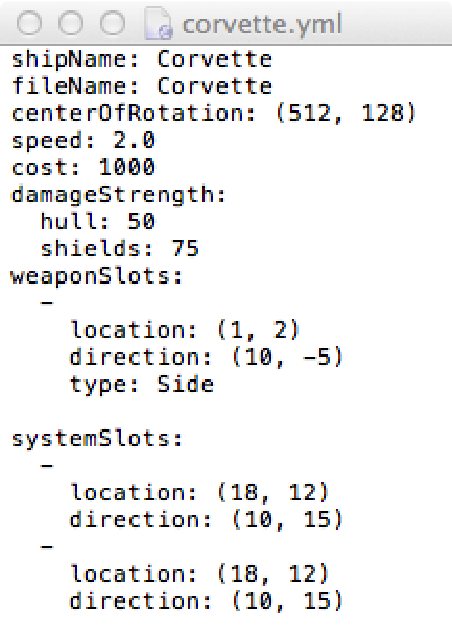
\includegraphics{res/configuration/corvetteYaml.pdf}
	\caption{
	example of ship class defined in yaml
	}
	\label{fig:configuration:corvetteYaml}
\end{marginfigure}


